\documentclass{article}
\usepackage[utf8]{inputenc}

\usepackage{amsfonts}
\usepackage{amsmath}
\usepackage[english]{babel}
\usepackage{booktabs}
\usepackage{caption}
\usepackage{csquotes}
\usepackage{enumitem}
\usepackage{float}
\usepackage{graphicx}
\usepackage{import}
\usepackage{multirow}
\usepackage{pdfpages}
\usepackage{rutitlepage}
\usepackage[subpreambles=false]{standalone}
\usepackage{subcaption}
\usepackage[flushleft]{threeparttable}
\usepackage{tikz}
\usepackage{tabularx}
\usepackage[colorinlistoftodos]{todonotes}

\usepackage[linesnumbered,ruled,vlined]{algorithm2e}
\newcommand\mycommfont[1]{\footnotesize\ttfamily\textcolor{blue}{#1}}
\SetCommentSty{mycommfont}

\usepackage[backend=biber,sorting=none]{biblatex}
\addbibresource{references.bib}

\usepackage{ftnright}
\renewcommand\footnoterule{{\hrule height 0.8pt}}

\usepackage{geometry}
\geometry{
   a4paper,
   left=20mm, right=20mm,
   top=20mm, bottom=25mm
 }
 
\usepackage{hyperref}
\hypersetup{
  colorlinks=true,
  citecolor=black,
  urlcolor=blue,
}

\usepackage{pgfplots}
\pgfplotsset{compat=1.3}
 
 
\setlength{\columnsep}{10pt}  % Default value: 35pt
\setlength{\tabcolsep}{2pt}  % Default value: 6pt
\renewcommand{\arraystretch}{1}  % Default value: 1


\begin{document}

   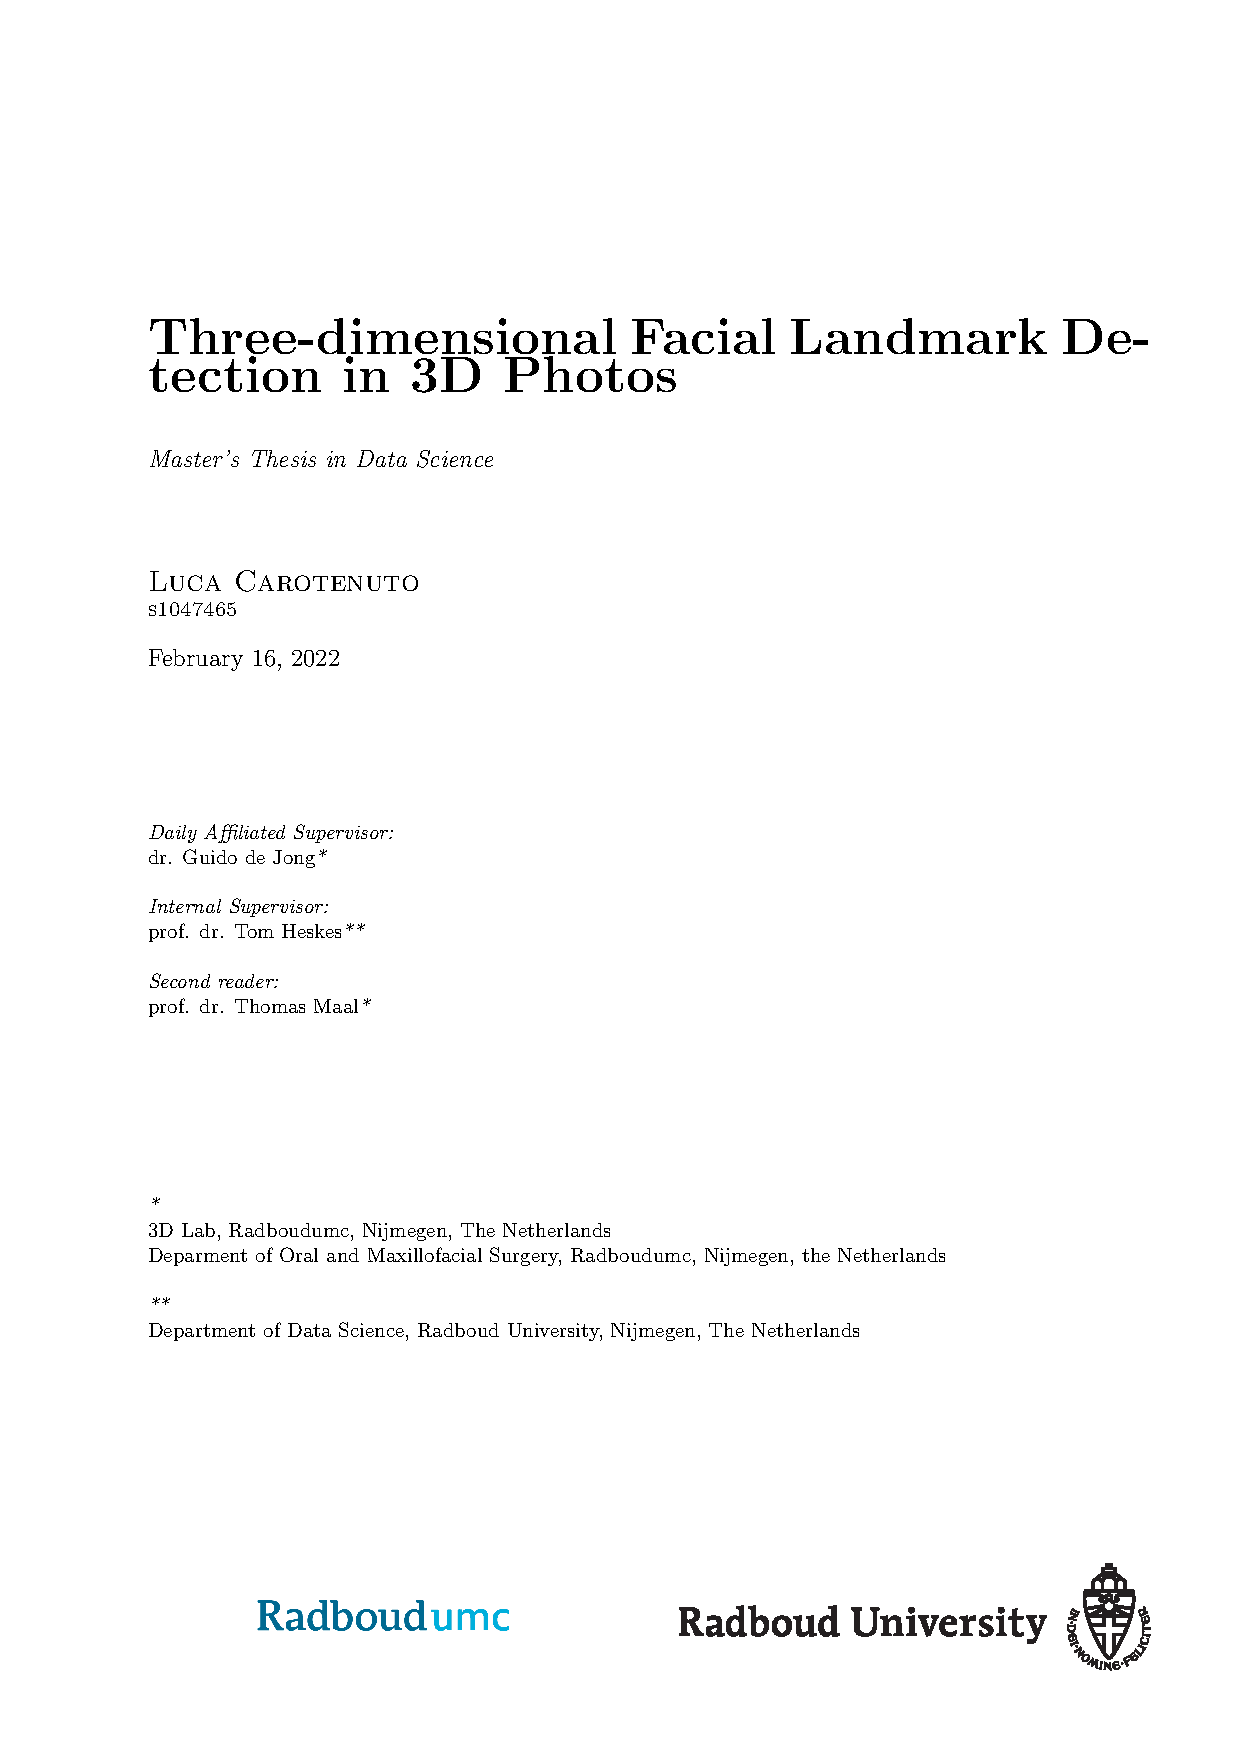
\includepdf[pages=-]{titlepage/titlepage.pdf} % create with pdfescape.com
 % \subimport{titlepage}{titlepage}

  \subimport{introduction}{abstract_thesis}
  \restoregeometry

\twocolumn
  \subimport{introduction}{introduction_thesis}
  \subimport{works}{works_thesis}
  \subimport{methods}{methods_thesis}
  \subimport{results}{results_thesis}
  \subimport{discussion}{discussion_thesis}
  \subimport{discussion}{conclusion_thesis}

\onecolumn
  \printbibliography
  \clearpage

\begin{refsection}

\twocolumn
\appendix
  \subimport{appendices}{1}
  \clearpage
\onecolumn  
  \printbibliography
\end{refsection}
    
\end{document}